\chapter{Background} 
\label{chapter-background} 

%----------------------------------------------------------------------------------------
%	SECTION 
%----------------------------------------------------------------------------------------

\section{Machine Learning}
Machine Learning is a subfield of Artificial Intelligence (see Figure \ref{fig:venn-diagram}) concerned with the design of algorithms that allow machines (e.g. computers, robots, embedded systems) to learn. For a task \textbf{T}, a performance measure \textbf{P} and an amount of data \textbf{D}, the system is said to be learning if it improves its performance \textbf{P} at the task \textbf{T} by increasing \textbf{D} (gain experience). Moreover, there are three main types of learning paradigms, namely supervised, unsupervised and reinforcement learning. In supervised learning \citep{supervised}, the model learns on a labeled dataset, providing an answer that the algorithm can use to evaluate its accuracy on training data. An unsupervised model \citep{unsupervised}, on the contrary, extracts features and patterns from unlabelled data. Lastly, reinforcement learning \citep{sutton} is typically used to train agents in dynamic environments, where the agent is able to act upon the environment. Reinforcement learning is best explained by an analogy. The learning algorithm is like a dog trainer, which teaches the dog (agent) how to respond to specific signs, like a whistle for example. Whenever the dog responds correctly, the trainer gives a reward to the dog, reinforcing the correct behaviour of the dog. Based on these three paradigms, several families of algorithms have been invented. Deep learning \citep{deeplearning-overview} is one of those families and is particularly powerful on perception tasks.
\begin{figure}[!ht]
\centering
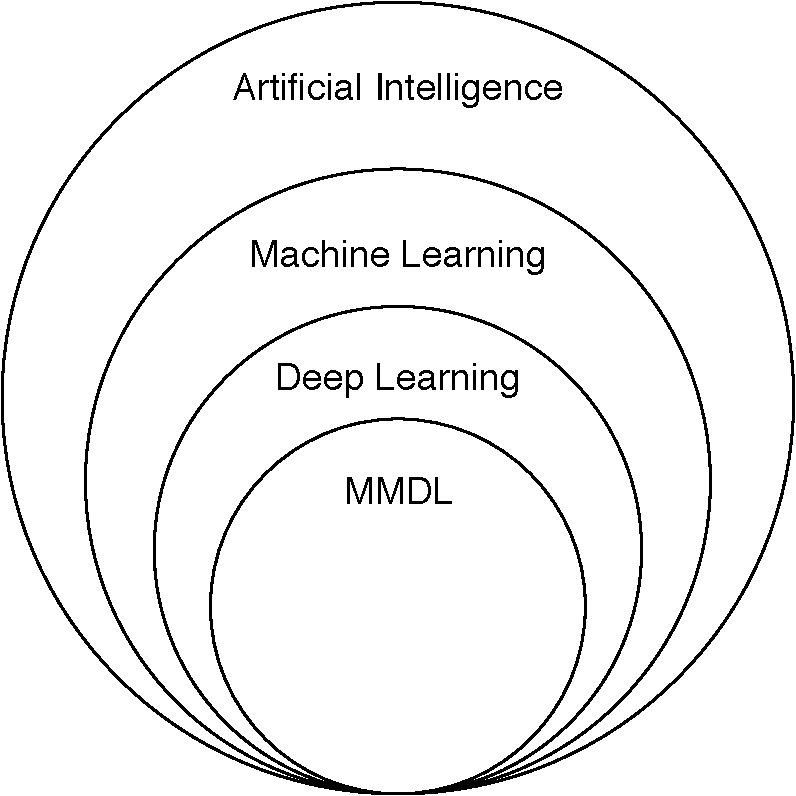
\includegraphics[scale=0.45]{figures/venn}
\caption{Venn diagram of the Artificial Intelligence field.}	
\label{fig:venn-diagram}
\end{figure}


%-----------------------------------
%	SUBSECTION 
%-----------------------------------
\section{Deep Learning}\label{sec:deep-learning}
Deep learning models, also called Deep Neural Networks, offer the significant advantage of being able to learn their own feature representation for the completion of a given task. A neural network is loosely inspired from our own brains, but can best be seen as a series of stacked non-linear parametric functions, enabling the network to learn multiple levels of representation with increasing abstraction. The parameters are tuned by optimizing a loss function with Stochastic Gradient Descent (SGD) or one of its many enhancements \citep{optim-algos}. Let $\bm{\theta}$ be the set of parameters, $\mathcal{L}$ the loss function, $y$ the groundtruth (labels) and $\hat{y}$ the predictions. First, the SGD algorithm estimates the gradient of the cost function on a randomly sampled batch of size $N$ as
\begin{equation}
\mathbf{g} = \frac{1}{N}\nabla_{\bm{\theta}}\sum_{i=1}^N\mathcal{L}(\hat{y}^{(i)},y^{(i)})
\end{equation}
where the computation of the gradient itself is done using back-propagation (BP) \citep{backprop}. The SGD algorithm then follows the estimated gradient downhill, $\bm{\theta} \leftarrow \bm{\theta} - \epsilon\mathbf{g}$ where $\epsilon$ is the learning rate, in the hope of minimizing the loss.

Optimizing the parameters to represent all valid inputs of a task, where the data is often very high-dimensional (e.g., images, sounds, text), may seem hopeless. However, neural networks surmount this obstacle by assuming that these high-dimensional data are lying along low-dimensional manifolds\footnote{A manifold designates a connected set of points that can be approximated well by considering only a small numbers of degrees of freedom.} \citep{goodfellow-book}. An intuitive observation in favour of this claim is that uniform noise essentially never resembles structured inputs from these tasks. More rigorous experiments supporting the manifold hypothesis are \citep{manifold-1, manifold-2, manifold-3}.


\subsection*{Multi-Modal Deep Learning}\label{sec:mmdl}
As a reminder, a modality refers to "the way in which something happened or is experienced" \citep{taxomany-multimodal}. Multi-Modal Deep Learning (MMDL) is simply the research area of neural networks using input samples consisting of multiple modes. Baltrušaitis et al. identified five non-exclusive use-cases of MMDL,
\begin{itemize}
\item \textit{Representation}: learning how to represent and summarize multi-modal data in a way that exploits the complementarity and redundancy
\item \textit{Translation}: learning how to map data from one modality to another (e.g., image captioning)
\item \textit{Alignment}: learning to identify the direct relationships between elements from two or more different modalities (e.g. alignment of sound and video)
\item \textit{Fusion}: learning to join information from two or more modalities to perform predictions 
\item \textit{Co-learning}: learning to transfer knowledge between modalities and their respective predictive models (e.g., zero shot learning)
\end{itemize}
The EMMA module is applied to multi-modal networks performing fusion. Furthermore, networks doing fusion can combine their modalities in three different ways: by early-fusion, late-fusion and an hybrid of the first two. Early-fusion architectures have uni-modal encoders extracting the features of each mode, the obtained features are then concatenated altogether and fed into a common decoder making the predictions (see Figure \ref{fig:early-fusion}). In contrast, late-fusion has uni-modal predictors for each mode, followed by a decoder weighting the uni-modal predictions to compute the final prediction. 
\begin{figure}[!h]
\centering
\begin{subfigure}{.45\textwidth}
\vspace*{15.5mm}
  \centering
  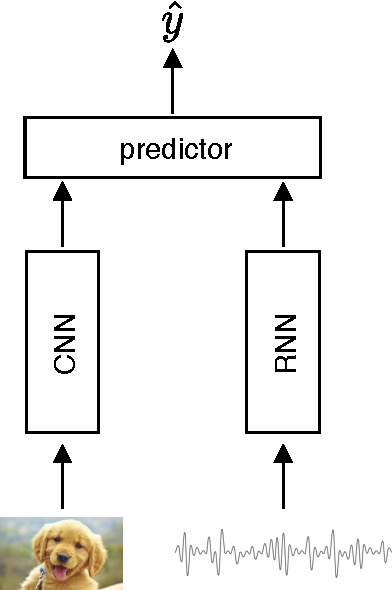
\includegraphics[width=.55\linewidth]{figures/early-fusion}
  \vspace*{3mm}
  \caption{Early-fusion}
  \label{fig:early-fusion}
\end{subfigure}%
\begin{subfigure}{.45\textwidth}
  \centering
  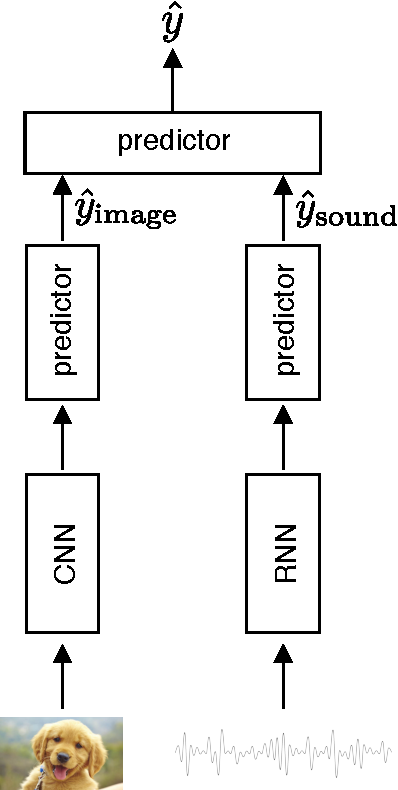
\includegraphics[width=.55\linewidth]{figures/late-fusion}
  \vspace*{2mm}
  \caption{Late-fusion}
  \label{fig:late-fusion}
\end{subfigure}
\caption[Early and late fusion]{Fusion of images and sounds for a classification task with a Convolutional Neural Network (CNN) \citep{image-recognition}, Recurrent Neural Network (RNN) \citep{machine-translation}.}
\label{fig:fusion}
\end{figure}


%----------------------------------------------------------------------------------------
%	SECTION 
%----------------------------------------------------------------------------------------
\section{Physics meets Deep Learning}\label{sec:ebm}
Modelling complex probability distributions by parametric functions such as deep learning models is a difficult task, because all the probabilities must be positive and sum up to one. At its origins, many researchers in deep learning had an academic background in physics, from which they regularly found inspiration to solve problems. An example of this is the distribution of kinetic energies among molecules of gas, called the Boltzmann distribution, and given by
\begin{equation}
p(E_i) = \frac{1}{Z}e^{-E_i/k_B T} \quad \text{with the partition function} \quad Z = \int e^{-E_j/k_B T}
\label{eq:boltzmann-distrib}
\end{equation}
where $E_i$ is the kinetic energy of molecule $i$, $k_B$ the Boltzmann constant and $T$ the temperature of the environment. The first thing to notice is that all the probabilities are positive and sum up to one for any set of combinations of energies $E_i$. Another observation to make is that high values of energies are unlikely ($E_i \propto -\log p(E_i)$), unless the temperature is sufficiently high enough. To sum it up, the Boltzmann distribution can be used to normalize any function to a distribution, where the temperature $T$ is a parameter influencing the entropy of the distribution. The Boltzmann distribution has two major applications in deep learning. First, it corresponds to the soft-max activation function \citep{softmax}, employed commonly for the purpose of outputting probabilities in multi-category classification tasks. Secondly, it was also used by deep learning researchers to construct energy-based models \citep{ebm-tutorial}. These types of neural networks optimize an energy function to be low on the data manifold and high everywhere else (see Figure \ref{fig:ebm-intervals}), which is the mapped to probabilities via the Boltzmann distribution. A few examples of efficient energy-based models are Generative Adversarial Networks (GAN) \citep{gan}, Variational Autoencoders (VAE) \citep{kingma-vae} and Denoising Autoencoders (DAE) \citep{dae-vincent}. The latter will be used in this work to measure the outlyingness of the data (see Chapter \ref{chapter-energy-estimation}).
\begin{figure}[!ht]
\centering
\includegraphics[scale=0.55]{figures/ebm-intervals-t}
\caption[Energy surface evolution]{The shape of the energy surface at four intervals. Along the x-axis is the variable X and along the y-axis is the variable Y . The shape of the surface at (a) the start of the training, (b) after 15 epochs over the training set, (c) after 25 epochs, and (d) after 34 epochs. The energy surface has attained the desired shape: the energies around the training samples are low and energies at all other points are high. \textit{Image and caption from} \,\citep{ebm-tutorial}.}
\label{fig:ebm-intervals}
\end{figure}